\documentclass{article}
\usepackage{amsmath}
\usepackage{graphicx}
\usepackage{amsfonts}
\usepackage{color}
\usepackage[utf8]{inputenc}
\usepackage[a4paper,left=2.5cm,right=2.5cm,top=2cm,bottom=2cm]{geometry}
\DeclareMathOperator{\Tr}{Tr}
\usepackage{hyperref}

\title{Homework 3, Fall 2025 18338}
\author{Due 10/9/2025 11:59pm}
\date{}
\begin{document}
\maketitle


\noindent{\large\color{blue} Please submit your homework via canvas.mit.edu. \\
If you are submitting .jl or .ipynb files, you must additionally submit .html or .pdf file that captures running notebook or code.}

Start thinking about a final project proposal.

\subsection*{Reading and Notes}
Read chapter 1, 2, 3 of the class notes, and optionally comment  by placing  issues on \verb+https://github.com/mitmath/18338/issues+.
Do not worry about missing references, typos are welcome, but what I really appreciate are
the high level style issues and the first point where things just do  not make sense.
Yes, these are harder, and more subjective, but in the end, more valuable.


\subsection*{Problem sets}
Do at least 7 out of the following 11 problems (Computational/Theoretical problems are denoted as C/T). Exercise with numbers and pages are from the class notes.

\subsection*{Concentration of Measure for Gaussian Ensembles}

It is remarkable how well the semicircle describes the histogram for Gaussian ensembles and other Wigner-type matrices. These mathematical and computational problems investigate the semicircle, how good it is, and how far off we can get. Section 1.1 and section 5 of reference \href{http://www-math.mit.edu/~edelman/homepage/papers/flucts.pdf}{http://www-math.mit.edu/~edelman/homepage/papers/flucts.pdf} are related to this question.

Take as given that the tridiagonal matrix $T_n$ when normalized by dividing by $\sqrt{n \beta }$ (i.e., $H_n = T_n/\sqrt{n \beta }$) on Page 109 (equation (6.3)) of the class notes has the same eigenvalues as a Gaussian ensemble, where any $\beta>0$ is allowed. 
This normalization approximately makes the 
eigenvalues in the interval $[-2,2]$ and the moments  Catalan numbers as $n \rightarrow \infty$.
Make use of \verb|Tridiagonal| in Julia, and use the following code snippet as a reference.

\begin{figure}[h]
    \centering
    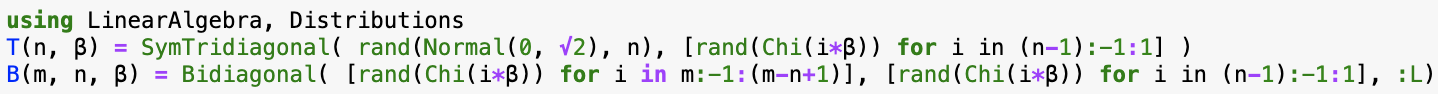
\includegraphics[width=6in]{code1.png}
\end{figure}

\begin{enumerate}
    \item (T) or (C) The first moment (and all odd moments) of the eigenvalues of the Gaussian ensembles has expected value 0. (This is a way of saying that $\mathbb{E}[\Tr(T_n)]=0$.) Theoretically or with a Monte Carlo simulation or both, conclude that $\Tr(T_n)$ is a scalar Gaussian. If you wish to access  Section 2.3.3 of Anderson, Guionnet, Zeitouni  \href{http://www.wisdom.weizmann.ac.il/~zeitouni/cupbook.pdf}{http://www.wisdom.weizmann.ac.il/~zeitouni/cupbook.pdf} (book page 42, pdf page 56) you might compare 2.3.10. How close are they?
    \item (T) or (C) The second moment of the eigenvalues can be obtained by adding the squares of the elements of the matrix and dividing by $n$.  Show that if we add the squares of the elements we obtain a random variable that is $\frac{2}{n\beta}$ times a chi-squared with
    $\beta(n(n-1)/2)+n$ degrees of freedom.   This is $C_1=1$ the first Catalan number.
Prove this by using simple properties of chi-square. (The degrees of freedom add.)  
If one wants to go further, one might use approximations such as if $X$ has the distribution of $\chi_k^2$ then $\sqrt{2X}$ is roughly normal with mean $\sqrt{sk-1}$ (or just $\sqrt{2k}$ with unit variance). Potentially compare the concentration of measure again.
    \item (T) What would happen in Problem 1 and 2 if the matrices are Wigner matrices (i.e., diagonal has variance 2 and the off-diagonal has variance 1) as $n\to \infty$? (Hint: use the Central Limit Theorem.)
    \item (C) Investigate how other odd moments deviate from 0 or how even moment deviate from the Catalan numbers. (i.e., How much do they differ from our expectations? Using Monte-Carlo, investigate what you see from the deviations.)
    \item (C) Try to investigate how the histograms themselves deviate from the semicircle. One can draw lots of pictures to see the semicircle. but what is interesting is to take averages and watch the fluctuations. See if you can estimate the fluctuations to the semicircle over various intervals using normals. One might start by taking the mean and seeing how far off finite $n$ is from infinite $n$, or one can consider the variance.
    \item (C) Perform Monte Carlo experiments on non-Gaussians carefully enough to predict the deviation.
\end{enumerate}

\subsection*{Laguerre ensembles and Others}

\begin{enumerate}
    \item (T) or (C) Perform Monte Carlo experiments to explore the mean and variance of the sum of the singular values of the bidiagonal model (Page 109  Equation (6.4)) ($m = n$) for different $n$'s. Furthermore, how does the sum change as a function of $\beta$? Is the mean monotonically going up or down? Where does it change? Again, use the Julia code in the first question as a reference.
    \item (T) or (C) Investigate numerically or mathematically the sum of the singular values for Laguerre ensembles normalized properly and see whether they converge monotonically in an increasing or decreasing manner.
    \item (C) Plot the histogram of the square singular values of (for different $z$'s on the complex plane)
        \begin{verbatim}
            (randn(n, n)+im*randn(n, n)) / sqrt(2*n) - z * I
        \end{verbatim} and compare $|z|<1$ with $|z|>1$.
    \item (C) Exercise 1.13 (page 29)
    \item (T) Exercise 2.7 (page 42)
   \item (T) or (C) Exercise 2.10 (page 43) (This is a good exercise, and can count as two problems!)
   
\end{enumerate}
 
\end{document}

